%\chapter{The Optimum Receiver}

%\subsection{Problem}
A single variable function $f$ is said to be convex if
%
\begin{align}
\label{ch1_convex_def}
f\sbrak{\lambda x + \brak{1-\lambda}y} \leq \lambda f\brak{x} + \brak{1-\lambda}f\brak{y}, 
\end{align}
%
for $\quad 0 < \lambda < 1$.
\begin{problem}
Execute the following python script. Is  $\ln x$ convex or  concave?
\end{problem}
%
\lstinputlisting{./chapter1/codes/1.1.py}
%
\begin{figure}[h]
\centering
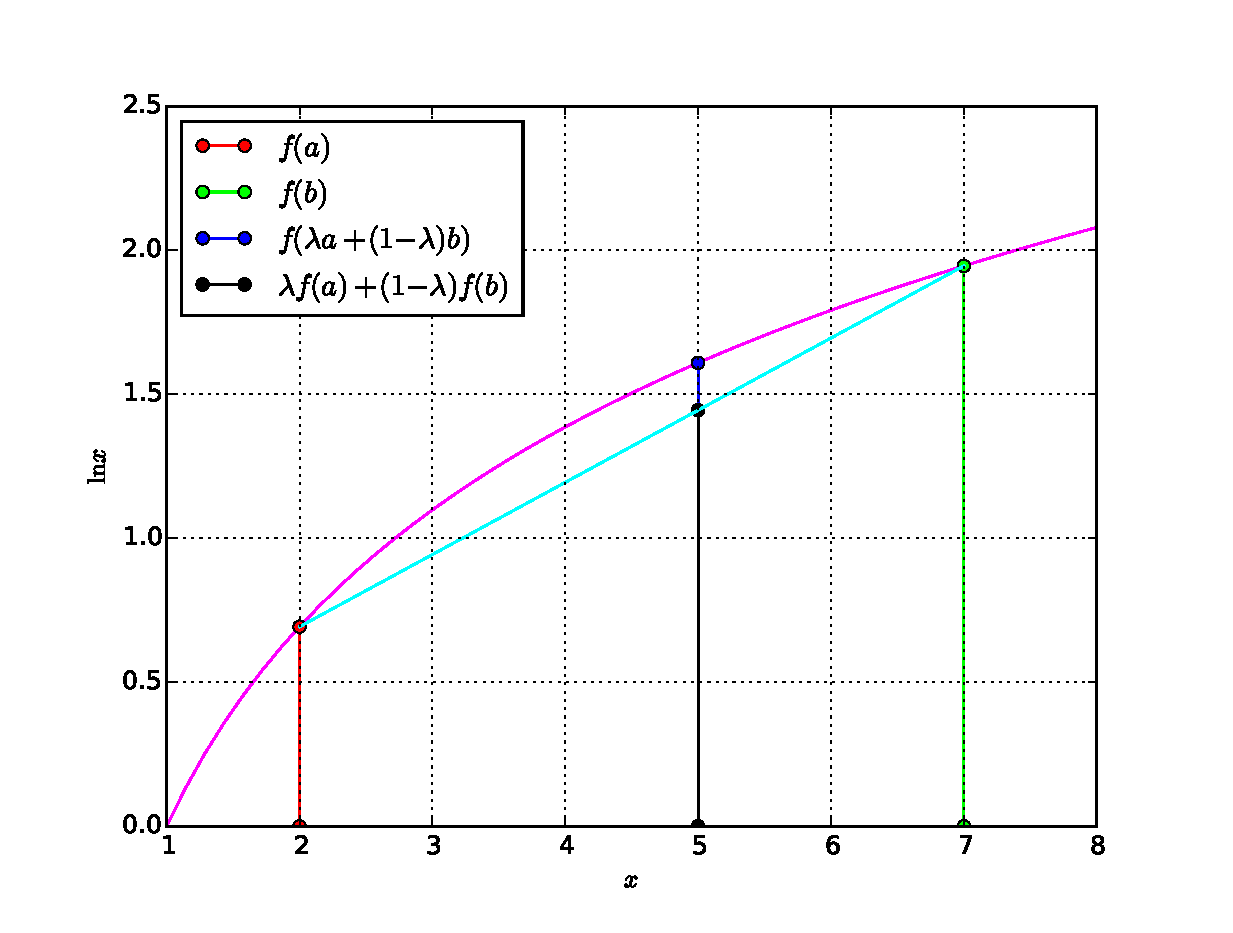
\includegraphics[width=\columnwidth]{./chapter1/figs/1.1.eps}
\caption{ $\ln x$ versus $x$}.
\label{fig.1.1}	
\end{figure}
%
\begin{problem}
Modify the above python script as follows to plot the parabola $f(x) = x^2$. Is it convex or concave?
\end{problem}
\lstinputlisting{./chapter1/codes/1.2.py}
%
\begin{figure}[h]
\centering
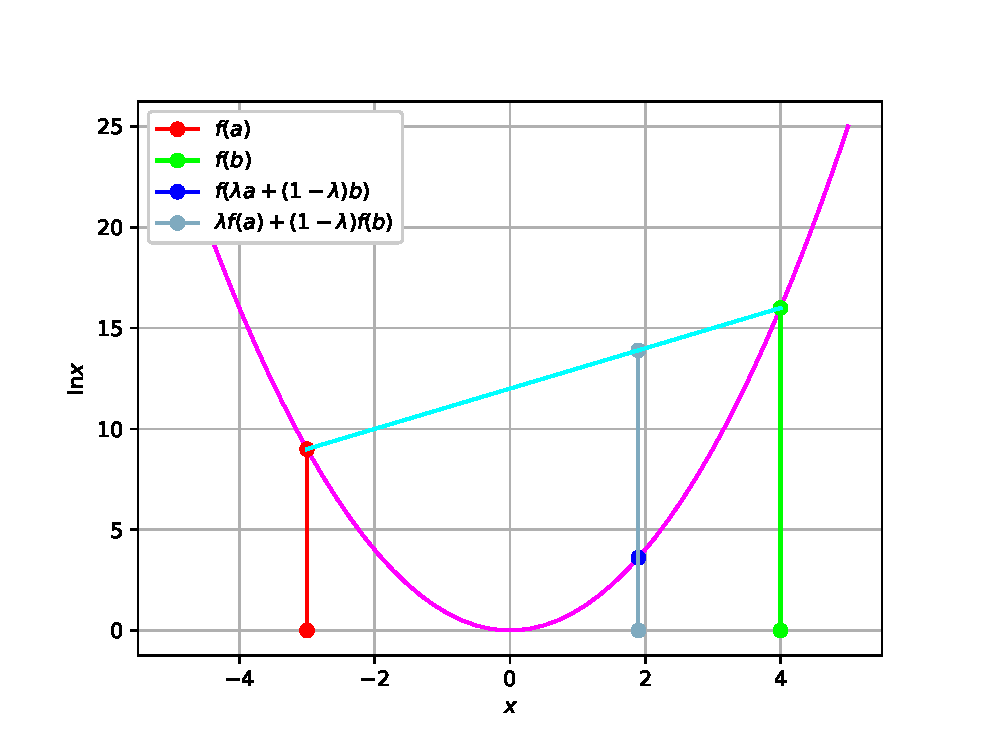
\includegraphics[width=\columnwidth]{./chapter1/figs/1.2.eps}
\caption{ $x^2$ versus $x$}.
\label{fig.1.2}	
\end{figure}
%
\begin{problem}
Execute the following script to obtain Fig. \ref{fig.1.3}. Comment.
\end{problem}
%
\lstinputlisting{./chapter1/codes/1.3.py}
%
\begin{figure}[h]
\centering
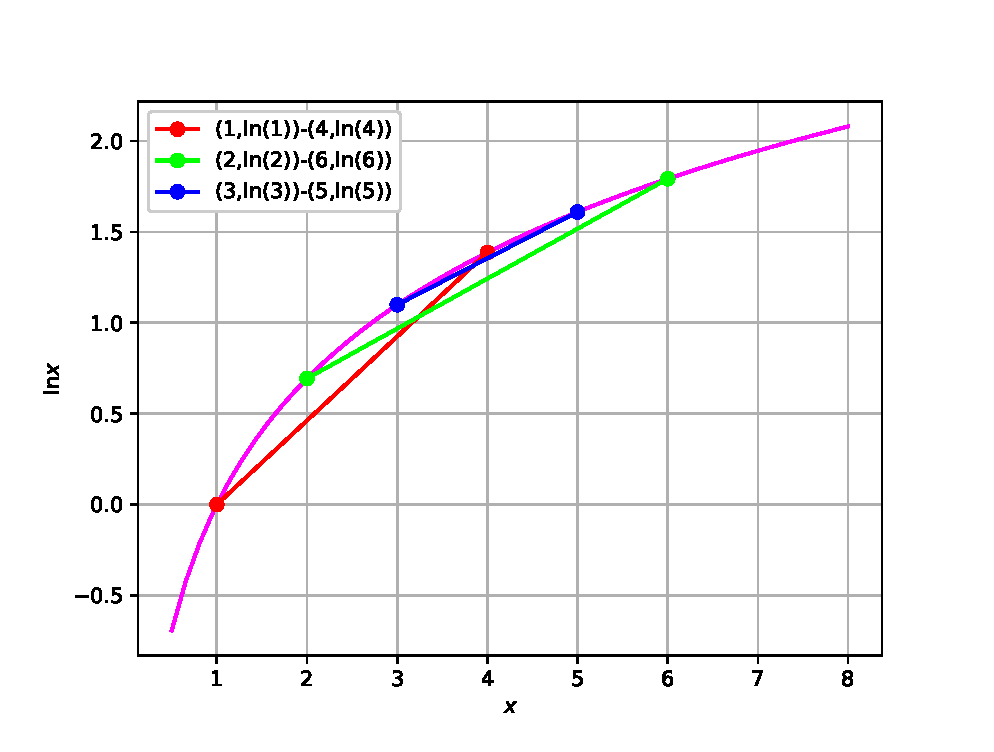
\includegraphics[width=\columnwidth]{./chapter1/figs/1.3.eps}
\caption{ Segments are below the curve}.
\label{fig.1.3}	
\end{figure}
%
\begin{problem}
Modify the script in the previous problem for $f(x) = x^2$.  What can you conclude?
\end{problem}
\begin{problem}
Let 
\begin{equation}
f(\mathbf{x}) = x_1x_2, \quad \mathbf{x} \in \mathbf{R}^2
\end{equation}
Sketch $f(\mathbf{x})$ and deduce whether it is convex.
Can you theoretically explain your observation using \eqref{ch1_convex_def}?
\end{problem}
%

